% Allow relative paths in included subfiles that are compiled separately
% See https://tex.stackexchange.com/questions/153312/

\providecommand{\main}{..}
\documentclass[\main/thesis.tex]{subfiles}

\onlyinsubfile{\zexternaldocument*{\main/tex/introduction}}

\begin{document}

\chapter{Implementation}

% \section{Approach}
% \subsection{ANN approaches}
% Numerous deep, neural network models have been proposed and utilized for the purpose of signal generation in recent years. WaveGans and WaveNet have been subject to significant improvements and experiments since their proposal \cite{nsynth2017,yamamoto2020parallel,oord2017parallel}. Even more recently Variational AutoEncoders (VAE's) have been utilized for generation of short percussive samples \cite{aouameur2019neural,ramires2019timbfeat}. In this work however, we opt to use digital signal processing methods to create a virtual synthesizer for the generation of audio signals as it provides several unique advantages:
% \begin{enumerate}[label=\roman*]
%   \item Fast, offline rendering of audio with no reliance on GPU: Currently not possible with state of the art models such as parallel WaveGan \cite{yamamoto2019parallel} and parallel WaveNet \cite{oord2017parallel}. 
%   \item Rendering at high sampling rates: Performance speed being a common issue, the standard sampling rate in most audio generation work utilizing neural networks appears to be under 24 khz \cite{yamamoto2019parallel,oord2017parallel,aouameur2019neural,ramires2019timbfeat}. However, a significant number of untrained human ears can detect a change in quality of audio between sampling rates of 192 khz and the industry standard of 44.1 khz \cite{reiss2016meta} with a dramatic increase in quality detection after training. Therefore we can safely assume that most producers would prefer their audio samples to have sampling rates of 44.1 khz or higher. In this work, we fix our sampling rate to the 48 khz standard. 
%   \item Neural networks are viewed as unexplainable black box solutions \cite{basheer2000artificial}. Some models such as VAE's can learn an underlying latent space of parameters and capture the distinguishing features of the different labels in a dataset. However, these spaces are learned in an unsupervised manner and must be manually analysed, perhaps extensively, before they can be understood \cite{esling2018generative}. The use of a virtual synthesizer for audio generation makes our parameters readily understandable and easily modifiable. \\
% \end{enumerate}

% Automatic programming of virtual synthesizers has also been a topic of interest. In early 2000s, Interactive Genetic Algorithms (IGA's) were utilized for the generation of new sounds with various sound-engines \cite{johnson1999exploring,dahlstedt2001creating}. More recent work by Yee-King et al. \cite{yee2018automatic} used Long short-Term Memory (LSTM) models and genetic algorithms to find the exact parameters used to create a group of sounds. The sounds approximated were made by the same virtual synthesizer, not an external source; making the eventual replication certain even with random search. Since this work appears more focused on pads and textures rather than drums, feature matching appears to not be concerned with the envelope of the sounds but rather the frequency content within arbitrary time windows. Yet another recent, impressive work by Esling et al. used a large dataset of over 10,000 presets for a commercial VST synthesizer to learn a latent parameter space which can be sampled for creation of new audio \cite{esling2019universal}. As stated before, our work explores the rapid approximation of percussion sounds with no previous knowledge about the sonic capabilities of our virtual synthesizer, exploring the actual parameter space rather than its latent representation.
\label{impl}

\section{Virtual Synthesizer}
\label{vs}
We used the python based Pippi library for sound generation\footnote{https://github.com/luvsound/pippi}. This library uses a C back-end and focuses on fast offline generation of audio signals. In our implementation a synthesizer can have any number of sub-modules. The parameters that deterministically dictate the output signal of the sub-module as well as the range of values each parameter can take are shown in table ~\ref{table:1}. We call this number the \textit{stack size}. For the range of parameters each sub-module can take we call the sets of parameters that characterize a synth's sub-modules a \textit{program} (analogous to a preset).  Each sub-module can make an audio signal with the length of 
% AH: Be consistent about synth, synthesizer, virtual synthesizer, Synth
0.1-1 second. If the synthesizer has a stack size of more than 1 these audio signals are overlapped and the total amplitude is normalized.

\begin{table}[h!]
\centering
\resizebox{\columnwidth}{!}{\begin{tabular}{ |c|c|c| } 
\hline
Parameters & Value Range & notes and constraints\\
\hline \hline
Attack & 0-3 & A-D-S-R values relative\\
Decay & 0-3 & relative to A-S-R\\
Sustain & 0-3 & relative to A-D-R\\
Release & 0-3 & relative to A-D-S\\
OSC type & sine,square,saw & tone type\\
IsNoise & boolean & whether to generate noise\\
Sample Length & 0-1 second & - \\
StartTime & 0-1 second & Length+Start<1\\
Amplitude & 0.1-1 & 1 = max amplitude\\
Pitches(notes) & list of pitches &  range of C0(16.35hz) to B9 \\
HP filter Cuttoff & 0-20000 & -\\
LP filter Cuttoff & 20000-HP & never lower than HP cutoff\\
Filter Order & 4,8,16 & butterworth filter order \\
\hline
\end{tabular}}
\caption{Synthesizer Sub-module Parameters. Despite the simplicity of the parameters and our efforts at constraining the ranges, the number of parameters that can be randomly chosen for each sub-module is in the order of $10^{15}$ }
\label{table:1}
\end{table}


\section{The Ear}

\begin{figure}[H]
\centering
\textbf{Visual Representation of Raw Features}\par\medskip
    \subcaptionbox{Recorded hat sample}{    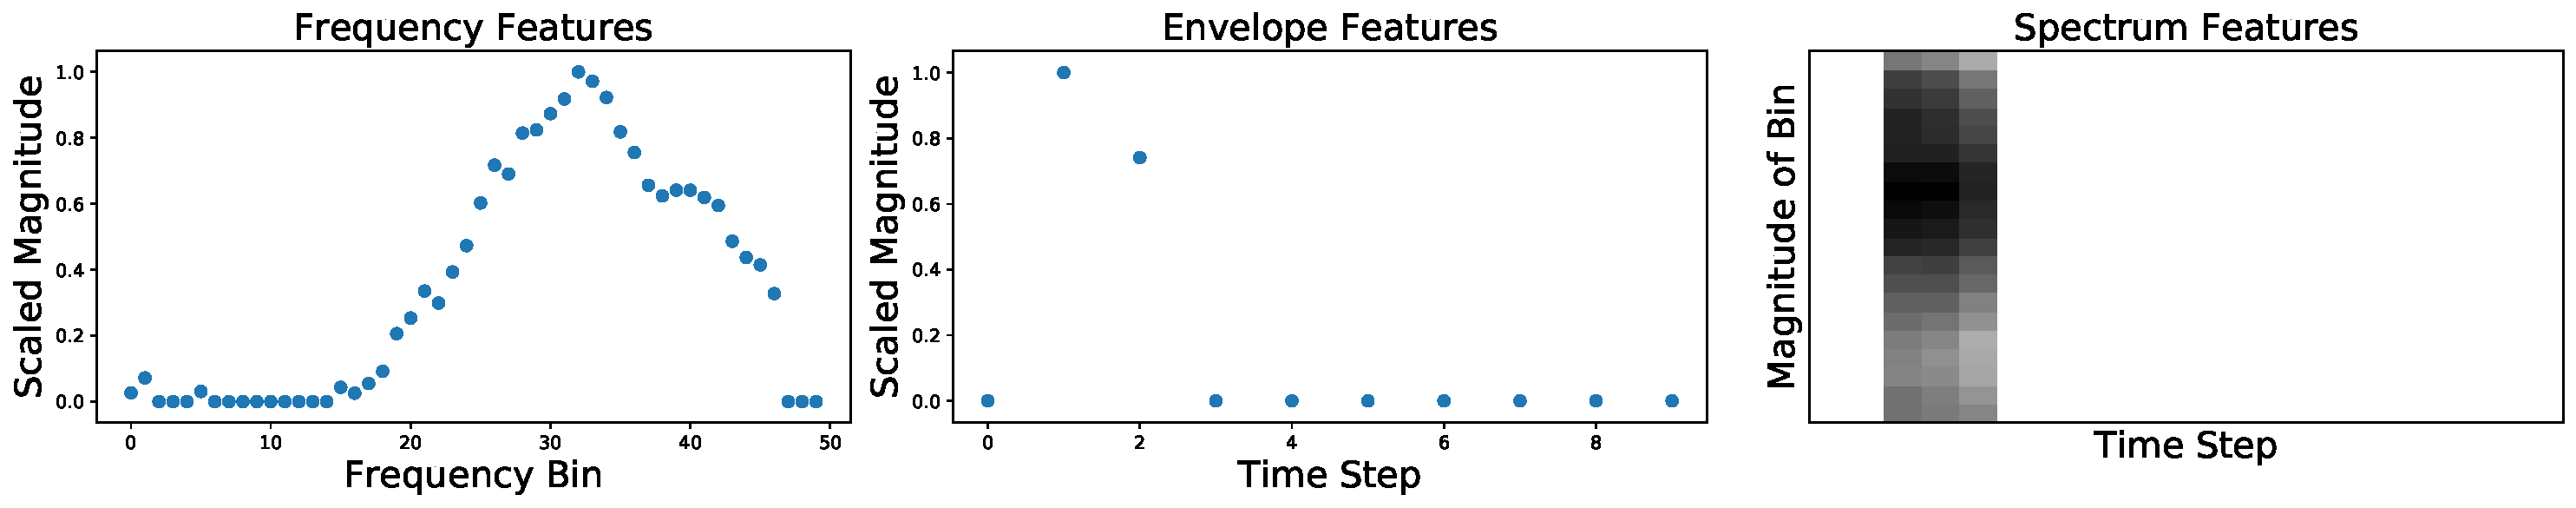
\includegraphics[width=1\columnwidth]{images/ff1.pdf}
    }
    \subcaptionbox{Randomly generated audio with percussive qualities, resembling a tight snare}{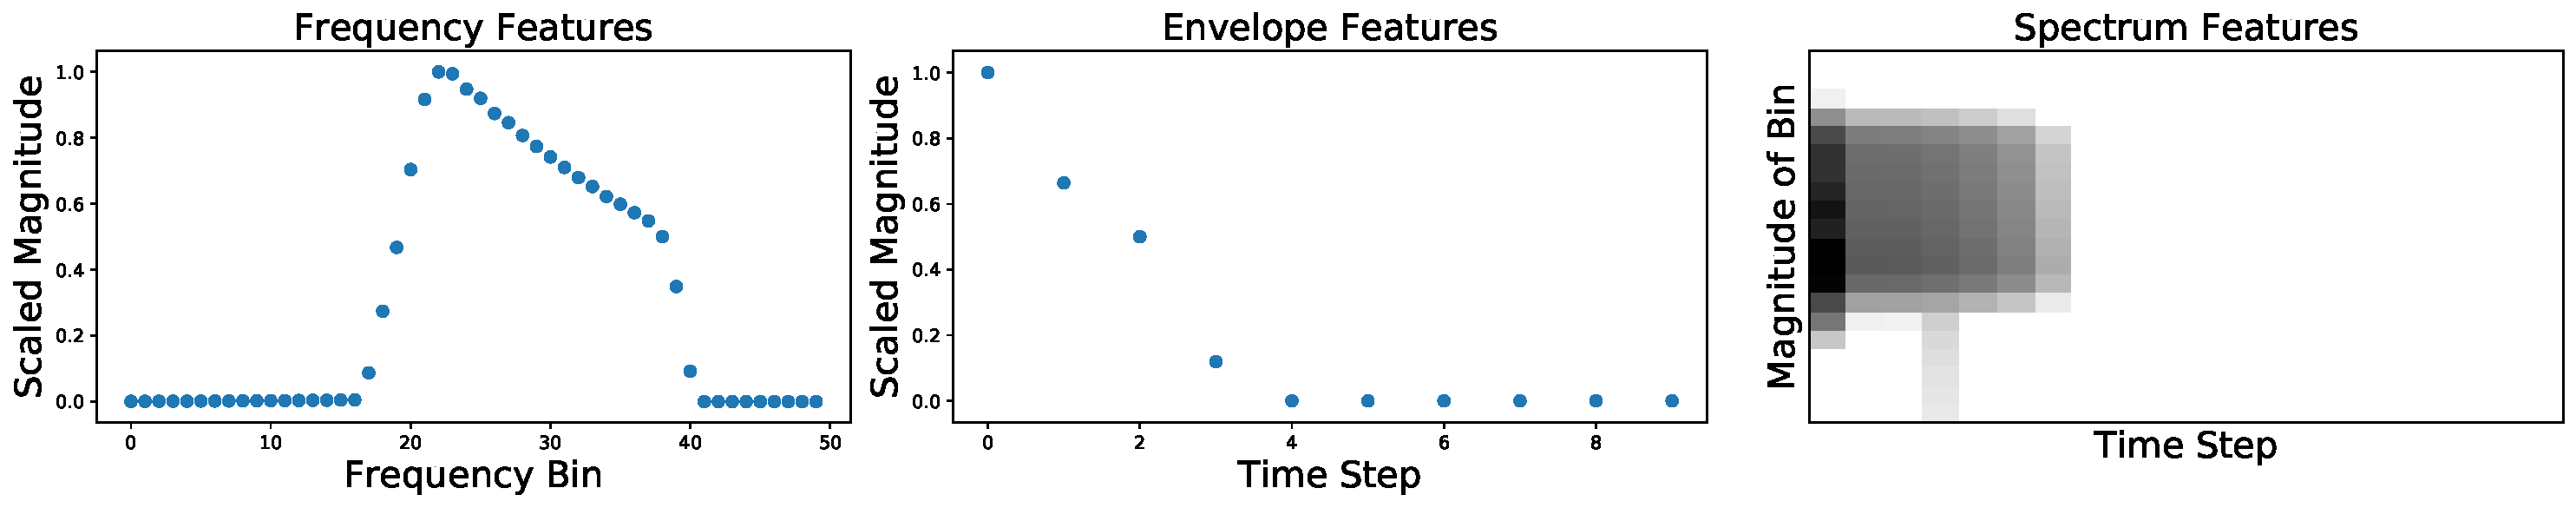
\includegraphics[width=1\columnwidth]{images/ff2.pdf}}
    \subcaptionbox{A randomly generated noise with a percussive envelop but non-percussive frequency features (modulated pitch)}
    { 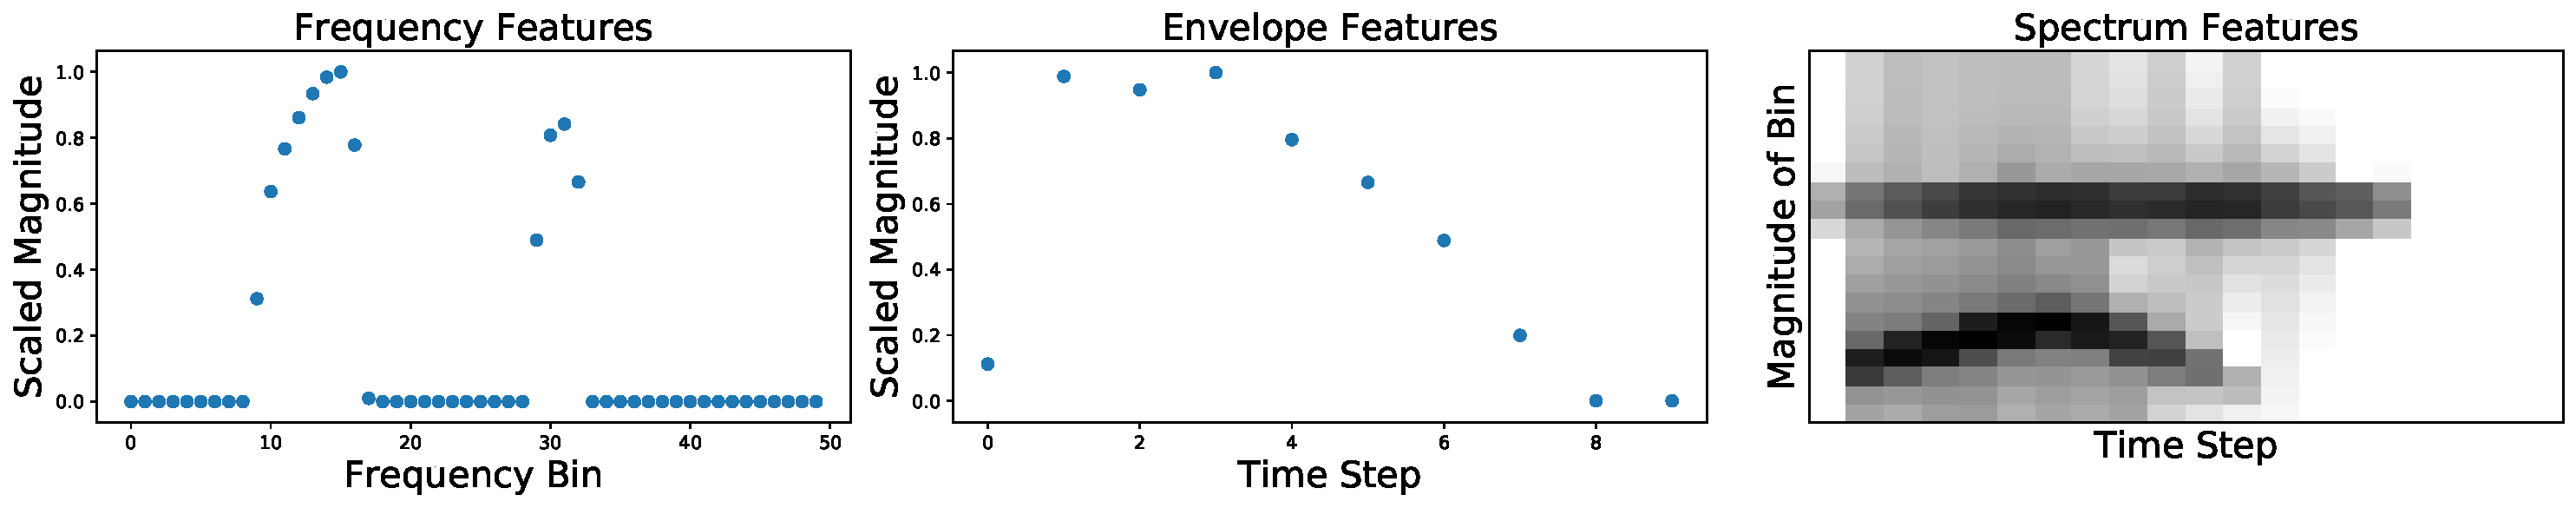
\includegraphics[width=1\columnwidth]{images/ff3.pdf}}
\caption{Graphed representation of features extracted for 3 different samples. Sample $a$ is a recorded hat from our database. sample $b$ is an example of randomly generated noise with percussive qualities that we found suitably similar to a snare sound. Sample $c$ is an example of a randomly generated noise where the spectrum features are necessary for proper classification.}
\label{fig:stackspectrums}
\end{figure}

What we refer to as an "ear" is any method (such as machine listening) of evaluating a piece of audio, capable of "listening" to a piece of audio and giving it a score (or a list of scores) based on how well it satisfies certain criteria. In this work we are mainly focused on percussive generation, therefore, what we require from the ear is to give us probabilities of an audio sample belonging to various categories. As our synthesizer outputs are close to deterministic for all programs, the evaluations of the ear would allow us to associate scores of the sound with the program that generated it. In section~\ref{gens} we discuss how these scores can be used to navigate synthesis towards parameters which give us the desired sonic output.

 With our dataset of labeled drum sounds, discussed in~\ref{data}, we can confidently categorized unlabeled drum sounds given that we know they are drum sounds. However, a major hurdle towards the implementation of a "drum from non-drum" recognizing ear is that the set of sounds that are not percussive is infinite. 

In our case, drum groups are an example of closed sets, since we believe that a sufficiently large sample pack can effectively describe common drum categories. However, effective representation of all possible non-drum sounds is not attainable via examples alone. We hypothesize that the implementation of our virtual ear falls outside the traditional categorization problem and within the "Open Set Recognition" domain. 

Traditional classification tasks often make the assumption the data points used for training the model and future unlabeled data will emerge from the same system of processes~\cite{geng2020recent,mundt2019open}. This assumptions requires that sufficient positive examples of all possible classes exist and are trained on. A well documented issue often addressed in works utilizing GANs is that such assumptions lead to scenarios in which networks will assign high categorization probabilities to nonsensical, out of context data which should be rejected rather than categorized~\cite{geng2020recent,mundt2019open,hassen2020learning}.  

Our work is based around random generation of a sound followed by 2 decisions: \begin{enumerate}
  \item Whether the sound could be used as a drum
  \item If it does sound like a drum, what type of drum should it be?
\end{enumerate}
The first decision requires knowledge of what drums \textbf{do not} sound like, or knowledge of an infinitely large set. It also means that the source of sounds used in training the model (organic drum sounds) will be fundimentally different from the source of unlabled sounds we wish to categorize (noise from a synthesizer).

Following this, 
\subsection{Embedding model}
% http://www.justinsalamon.com/uploads/4/3/9/4/4394963/cramer_looklistenlearnmore_icassp_2019.pdf says they need almost 40 million samples 
% http://www.cs.toronto.edu/~zemel/documents/prototypical_networks_nips_2017.pdf
\subsection{Two Phased model}
\label{sec:ear}
\subsubsection{Feature Extraction}


   % AH: is the virtual synthesizer a synth or a synthesizer that makes synthesizer
  % AH: you should make it 1 instance of a generated synth 
We only consider 1 second long sounds made with a single stacked synth, yet the set of possible synthesizer parameters (and we assume, the sound generated by the synth given these parameters) is extremely large. In our case, as discussed in Section ~\ref{survey}, the majority of sounds generated by the synth do not resemble percussion.  We determined that there are 2 steps necessary to effectively extract percussive sounds
from the randomly generated sounds produced by virtual synthesizers: 
\begin{enumerate}
   \item  Phase $1$: Binary separation of sounds with percussive features from non-percussive sounds.
   \item Phase $2$: Given confidence that the sound being categorized is percussive, categorizing its type.
\end{enumerate}
We are interested in extracting generalizable, domain agnostic features. In this work we rely entirely on Fast Fourier Transform (FFT) and by extension Short-time Fourier Transforms (STFT) for feature extraction. Using FFT, a signal can be represented by a vector with each index corresponding to a frequency-bin (a range of frequencies too close to be distinguishable) and the value at each index corresponding to the combined-magnitude of the frequencies within the bin. STFT can be employed when a more accurate representation is desired; via the application of the FFT to a sliding time-window on the signal to create a matrix (a list of vectors). This matrix can effectively represent the frequencies present in the signal at each time step, given the right window-length and hop-size (how much the window is shifted at each time-step).

% AH: If you need space shorten this paragraph to we use STFT which has worked in past and we use spectral-centroids and zero-crossings
Various works have demonstrated effective reconstruction of signals given their STFT~\cite{nawab1983signal,griffin1984signal}. For our purpose, if the original signal can be faithfully reconstructed from its STFT, analysis of the STFT may be relied on as source of fundamental features necessary for audible signal categorization. In the interest of keeping the feature space small and fundamental, other methods of feature extraction such as Spectral-Centroids~\cite{schubert2004spectral} and Zero-Crossing Rates~\cite{gouyon2000use} are not utilized.

Using only the STFT of signals as source of feature extraction we defined 3 transformation functions which we believe to capture important, unique attributes of percussive sounds.  These functions were applied at training time to 1 second audio samples before being sent to a classifier; transforming a signal into a set of features which we hope can capture the necessary information for our categorization task. 


\begin{enumerate}
\item Envelope Transformation: The goal of this feature is to capture the changes in loudness for the duration of the signal. Using STFT we generate a matrix $M_{i \times j}$ with rows $i$ and columns $j$ corresponding to time steps and frequency bins respectively, and with values $v_{i \times j}$ indicating the magnitude of the frequency bin $j$ at each time-step $i$. Information about the envelope of the signal can be extracted by summing the values of $M$ for each time-step (or row $i$), giving us a feature vector $v_i$. This vector is then normalized to the range of 0 to 1. The information contained in this vector is similar to that of a Root-Mean-Square measurement.
\item Frequency Transformation: A static, normalized snap-shot of the the frequencies present within the audio. The calculation of this feature vector is similar to the envelope, but the summation is done along the frequency axis. Another important distinction is that since capturing an adequate frequency resolution is important for this transformation, we utilized shorter hop-sizes and wider windows. A Mel Scale transformation was also applied in hopes that the captured features better represent human perception of frequencies. 
\item Spectrum Transformation: This function is simply a Mel Scaled STFT with its values normalized from 0-1. Since this features is a 2D matrix rather than a vector it captures more information about our signal but requires heavier, more complex computational methods to be utilized. 
\end{enumerate}

\subsection{The Models}
Using the described features, we trained several neural network models for Phase 1 and 2 in the Pytorch environment. The task of Phase 1 is to separate drums from not-drums (DrumVsNotDrum, or DVN). The task of Phase 2 is to categorize drums and percussion (DrumVsDrum, or DVD). We kept our feature space small, making it viable for feature selection and model design to be done on a trial and error basis. For all models, accuracy is calculated by prediction of all test dataset labels and the loss function and optimizer are Categorical-CrossEntropy and Adam respectively. Training continues until no reduction in loss and accuracy is observed in 10 epochs.  All activation functions are PReLU:
\begin {enumerate}
\item FC-DVN: Fully connected network trained on Envelope features, reaching 97\% accuracy on our test data for Phase 1. With size of 10x5x10.
\item CNNLSTM-DVN: A combination of CNN and LSTM models, where the CNN model extracts higher level features that are fed temporally to an LSTM cell. This model is trained on spectrum data and reaches 98\% accuracy on our test set. Its structure is the combination of a CNN with 2 output channels and kernel size $(7,3)$; Followed by an LSTM model of hidden size 800 and a fully connected layer of size 20x2.
\item E+F-DVD: A fully connected model trained on a concatenation of envelope and frequency features. Reaching 80\% accuracy for 6-way drum categorization in Phase 2. Size of 50x10x2x6.
\item CNN-DVD: A CNN model trained on Spectrum features. Reaching 82\% accuracy in a 6-way drum categorization in Phase 2. A combination of a CNN model with output channel size of 4, kernel of size of 5, another CNN model with output channel size of 8 and kernel of size 3. Followed by a fully connected network of shape 100x20x6.
\item FC-DVD: Fully connected 3 layer neural net with 78\% accuracy for 6-way drum categorization in Phase 2. Size of 400x200x50.
\end{enumerate}
The parameters are hand-picked and un-tuned. As discussed in section ~\ref{survey}, higher accuracy rates in these models do not translate to higher agreeableness with humans. leading us to believe that model accuracy on test data alone cannot be relied upon when the domain of sounds 
being categorized is switched from original percussion samples to virtual synth sounds.

With our models showing high accuracy on testing data, we combine models in order to increase the efficacy of each phase and address the "open set problem" for our task. For Phase 1 we only determine sounds as percussive if both FC-DVN and CNN-LSTM have determined it as such with over 90\% confidence. For the majority of our random generations that is not the case, but if a randomly generated sound has passed this phase, our three categorizers assign their categorizations to this sound. These categorizers have a moderate degree of agree-ability as seen in ~\ref{survey}, but often the decision is not unanimous. The fourth method of categorization, "averaged-cat", is implemented by taking the sum of the softmax outputs of all three categorizers, using it to determine the category. 

These models can be combined and weighted in various ways and the confidence thresholds can be modified in order to implement "virtual ears" with different properties. A glaring issue in the current implementation is the treatment of softmax outputs as a reasonable measure of a model's confidence. Ignoring that some models may have unwarranted higher confidence in their scores, skewing attempts at finding a consensus. 




\section{Data And Project Replication}
\label{data}

Our data is a large set of drum samples aggregated from personal libraries, free drum kits from the sample-swap project \footnote{https://sampleswap.org/} which we further processed to suit our categories, and a large set of drum sounds aggregated from royalty free sources such as musicradar \footnote{https://www.musicradar.com/}. We have made our dataset of free-drum sounds available for download. The scripts used to download and process royalty free samples will also be made available. Further information about downloading our dataset can be found on this project's github page. 

Our drum categories are claps, hats, kicks, rims/other, shakers, snares and toms. Other categories are chopped guitars, chopped pianos and n-stack-synths (random noise generated by the virtual synth with stack size of n, see ~\ref{vs}), utilized for learning percussive vs non-percussive sounds. Stack sizes refers to how many synth functions are connected together in a synthesizer.
Some notes about our dataset:


\begin{itemize}
\item Of the 6000 drum-sounds utilized in our work, the kick, snare and hat categories have the largest share at around 20\% each, while the shaker and rim (other) categories have the smallest at 5\% combined. Due to this we only focused on learning from kicks, snares, toms, claps and hats for Phase 1 of training (along with non-percussive groups of sound) ~\ref{sec:ear}.

\item For Phase 2 of training we only focused on categorizing snares, claps, kicks, hats and other (percussive sounds such as shakers, rims and unusual percussions that we couldn't categorize were grouped into this category). Non-percussive datasets were not used for this phase. 
\item In order to offset bias from data imbalance during training of our models, the categorical cross entropy loss was weighted by the group sizes. 
\item For any given model, 80\% of our data is used for training and 20\% is used for testing. 

\item We limit the size of the n-stack-synths category to 50\% of the total size of our drum dataset. This is done in order to measure whether the features extracted can address the "Open Set Recognition" problem, which will be discussed further in Section ~\ref{sec:ear}.
\end{itemize}
\end{document}